\chapter{Ewaluacja sprzętowa i optymalizacja}
\label{cha:Optymalizacja}
% Ewaluacja po implementacji sprzętowej. 
% Optymalizacja fps / energii.

% Wyznaczony model sieci \emph{LittleNet} w rozdziale \cite{ch:LN} został zaimplementowany sprzętowo co zostało omówione w  
W rozdziale \ref{ch:LN} wyznaczono model sieci \emph{LittleNet}. 
Architektura ta osiąga wartość $IoU = 0.71$ (dla zbioru testowego). 
Sieć została zaimplementowana sprzętowo co omówiono w rozdziale \ref{cha:Implementacja}.
Rozwiązanie to jednak należy sprawdzić pod kątem dokładności detekcji (poprawności z modelem programowym), przepustowości oraz zużycia energii, a także dokonać próby optymalizacji ich optymalizacji. 


\section{Ewaluacja}
Celem sprawdzenia zaprojektowanego rozwiązania wykorzystano zaimplementowaną aplikację sterującą (rozdział \ref{ch:sterowanie}).
Aplikacja pozwala na pomiar czasu przetwarzania oraz pomiar energii.
Aby możliwe było sprawdzenie dokładności otrzymanych rezultatów zaimplementowano funkcję obliczającą wartość metryki $IoU$ względem wartości referencyjnych.

Wstępne wyniki ewaluacji dawały inne rezultaty niż model programowy.
Dalsza analiza pozwoliła stwierdzić, iż model programowy wykorzystywał operacje zmiennoprzecinkowe do przeskalowania rozmiaru obrazu wejściowego.
Wykorzystanie do tego celu liczb całkowitych nieznacznie pogorszyło wynik.
Finalnie oba modele dawały identyczne rezultaty w postaci $IoU = 0.7015$, 
Wykorzystano tutaj ośmiokrotne zrównoleglenie warstw \emph{PW} pozwalające na osiągnięcie średnich wartości przepustowości $fps = 52.5$ oraz zużycia energii $e = 3652 J$ (wartość dla $52 500$ obrazów). 
Uzyskana dokładność oraz przepustowość pozwalają na osiągnięcie maksymalnych wartości funkcji \eqref{eq:iou_score} oraz \eqref{eq:fps_score}.
Na rysunku \ref{fig:results} przedstawiono rezultaty detekcji dla wybranych obrazów wchodzących w skład zbioru testowego.

\begin{figure}
    \centering
    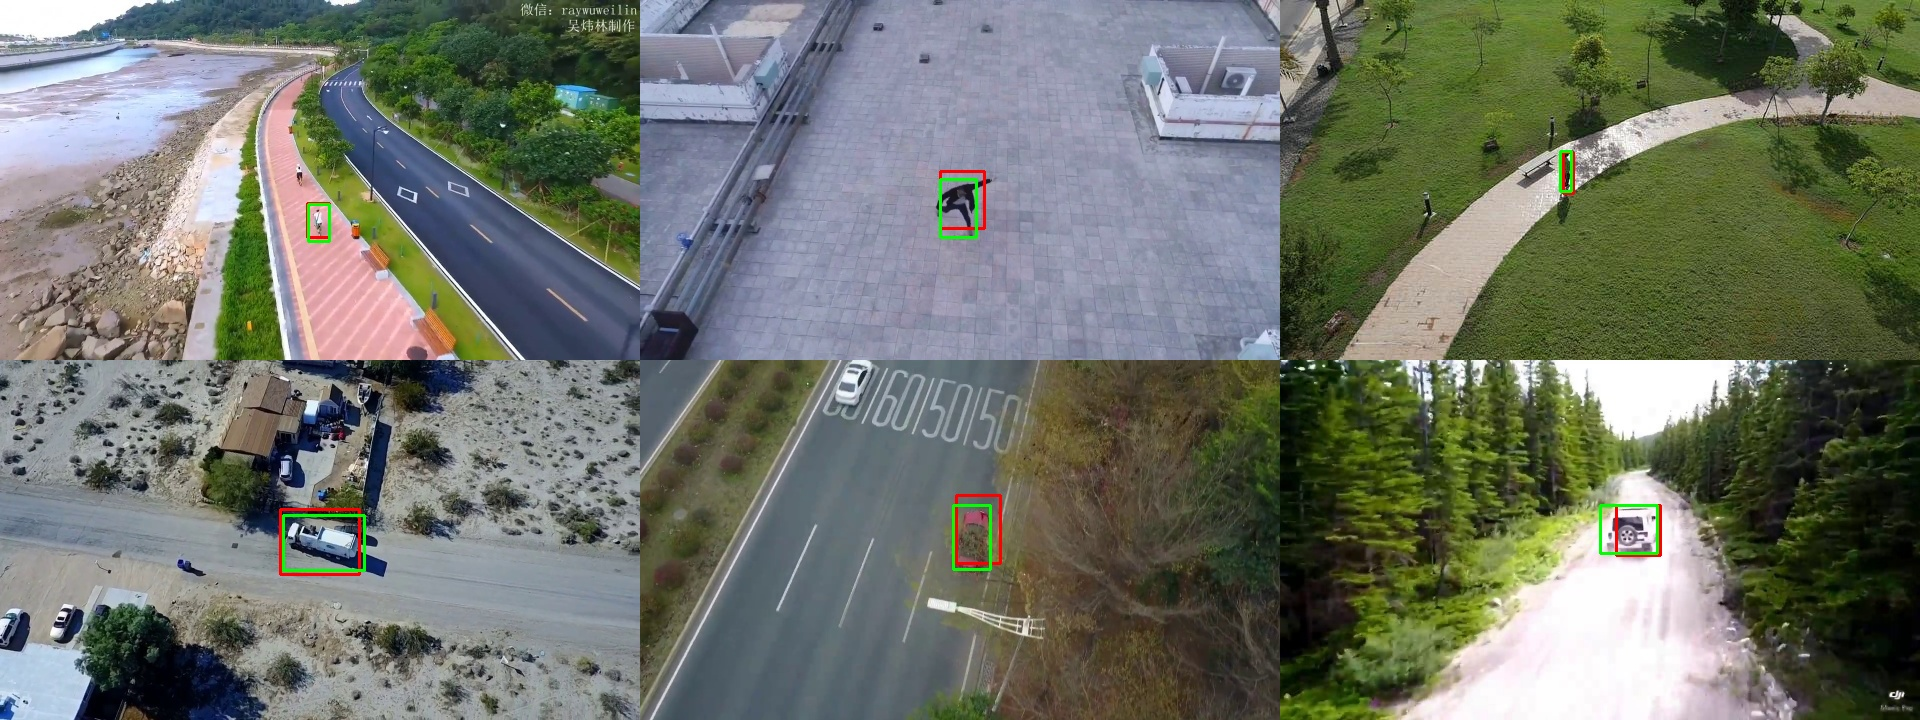
\includegraphics[width=0.9\linewidth]{images/results.png}
    \caption{Uzyskane rezultaty detekcji dla wybranych obrazów zbioru uczącego. 
    Źródło: \cite{dac_sdc_2021}.}
    \label{fig:results}
\end{figure}

\section{Optymalizacja}
Zakładając, iż otrzymana dokładność detekcji została by osiągnięta na zbiorze tajnym, optymalizacja może zostać ograniczona jedynie zmian parametrów akceleracji, takich jak zrównoleglenie $p$ warstw \emph{PW} czy częstotliwość zegara $f$ dla logiki programowalnej (dotychczas używana była częstotliwość $100$ MHz).
Łączną moc układu można wyrazić wzorem \eqref{eq:power}, gdzie $P_{PL}(p,f)$ to moc logiki programowalnej oraz $P_{PL}(p,f)$ moc układu procesorowego.
\begin{equation}
P(p,f) = P_{PS} + P_{PL}(p,f)
\label{eq:power}
\end{equation}
Zużycie energii $e$ układu potrzebnej do przeprowadzenia procesu detekcji $N$ obrazów osiągające przepustowość $fps(p,f)$ definiuje równanie \eqref{eq:energy}.
\begin{equation}
e(p,f) = \frac{N}{fps(p,f)}(P_{PS} + P_{PL}(p,f))
\label{eq:energy}
\end{equation}

Ponadto przybliżoną moc $P_{PL}(p,f)$ wyrazić można przez \eqref{eq:ppl}, zakładając liniowy przyrost mocy od $p$ dla warstw \emph{PW} oraz zależność mocy od częstotliwości przyjmując za $\beta(f)$. Przez $P_{DW}$ oraz $P_{PW}$ oznaczono moc akceleratorów odpowiednio \emph{DW} i \emph{PW} (dla akceleracji z użyciem tylko jednego \emph{PW\_PU}).
\begin{equation}
P_{PL}(p,f) = \beta(f) (P_{DW} + p P_{PW})
\label{eq:ppl}
\end{equation}

Przybliżony stosunek czasu trwania obliczeń warstwy \emph{DW} do czasu trwania całego cyklu przetwarzania wyrażono poprzez $\alpha(p)$. 
Wartości stałe stanowią liczbę maksymalnych wymaganych odczytów z pamięci RAM dla  warstw \emph{PW}(10 444 800) oraz \emph{DW}(460 000).
\begin{equation}
\alpha(p) = \frac{460 000}{460 000 + \frac{10 444 800}{p}} = \frac{p}{p+22.7}
\label{eq:alpha}
\end{equation}

Z równia \eqref{eq:alpha} można stwierdzić, iż znaczna część czasu przetwarzania przypada na akcelerację warstw \emph{PW} ($\alpha(1) = 0.04$, $\alpha(8) = 0.26$,  $\alpha(16) = 0.41$).
Tym samym zakładając \eqref{eq:fps}, gdzie $f_0$ oraz $fps_0$ to stałe.
\begin{equation}
fps(p,f) = p*\frac{f}{f_0}* fps_0
\label{eq:fps}
\end{equation}

Równanie zużycia energii przybiera postać \eqref{eq:energy_simple}.
\begin{equation}
e(p,f) = \frac{N}{p*\frac{f}{f_0}* fps_0}(P_{PS} + \beta (f) P_{DW} + p \beta (f) P_{PW})
\label{eq:energy_simple}
\end{equation}

Przyjmując $f$ jako stałą oraz zrównoleglenie $p_1$ oraz $p_2$ takie, że $p_1 < p_2$ 
to stosunek zużytej energii $e_2$ dla  $p_2$ do zużytej energii $e_1$ dla  $p_1$ wyznaczany jest przez \eqref{eq:e_cmp}.
\begin{equation}
\begin{aligned}
\frac{e_2}{e_1} = \frac{e(p_2)}{e(p_1)} &= \frac
{\frac{1}{p_2}(P_{PS} + \beta(f) P_{DW} + p_2 \beta(f) P_{PW})}
{\frac{1}{p_1}(P_{PS} + \beta(f) P_{DW} + p_1 \beta(f) P_{PW})}\\
&= \frac
{\frac{C_1}{p_2} + C_2}
{\frac{C_1}{p_1} + C_2}
\end{aligned}
\label{eq:e_cmp}
\end{equation}
 Większe zrównoleglenie przyniesie mniejsze zużycie energii, gdy $\frac{e_2}{e_1} < 1$ co jest prawdziwe dla każdego $p_2 > p_1$. 
 Wnioskując im wyższy stopnień zrównoleglenia tym mniejsze zużycie energii.
 W tym celu ustalono $p = 16$ oraz przeprowadzono ewaluacje.
 W rezultacie uzyskano $fps = 72.7$ oraz zużycie energii $e = 2739 J$.
 Co jest zgodne z wyznaczonymi nierównościami, pomimo zastosowania znacznych przybliżeń.
 
 Dla \eqref{eq:energy_simple} przyjmując $p$ jako stałą oraz przyjmując $P_{PL}$ jako moc dynamiczną bez straty ogólności (nie znana jest moc $P_{PS}$), wówczas zależność mocy od częstotliwości może zostać wyrażona poprzez \eqref{eq:dynf} \cite{dynamic_power} oraz zużycie energii poprzez \eqref{eq:energy_simple_f}. 
\begin{equation}
\beta(f) = \frac{f}{f_0}
\label{eq:dynf}
\end{equation} 
\begin{equation}
e(p,f) = \frac{N}{p*\frac{f}{f_0}* fps_0}(P_{PS} + \frac{f}{f_0} P_{PL})
\label{eq:energy_simple_f}
\end{equation}

Przyjmując dwie częstotliwości $f_1$ oraz $f_2$ takie, że $f_2 > f_1$, możliwe jest zmniejszenie zużycia energii, gdy spełniona jest zależność \eqref{eq:cmp}.
\begin{equation}
e(p, f_2) < e(p,f_1)
\label{eq:cmp}
\end{equation}
\begin{equation}
\frac{1}{f_2}(P_{PS} + \frac{f_2}{f_0} P_{PL}) < 
\frac{1}{f_1}(P_{PS} + \frac{f_1}{f_0} P_{PL})
\end{equation}
\begin{equation}
\frac{P_{PS}}{f_2} < 
\frac{P_{PS}}{f_1}
\end{equation}
\begin{equation}
f_1 < f_2
\end{equation}
co jest zawsze prawdziwe.
Wnioskując im większa częstotliwość przetwarzania, tym mniejsze zużycie energii.
Wartość częstotliwości musi jednak zapewniać prawidłowe wykonanie obliczeń.
Ponadto niejawnie zakładano, iż część przetwarzania realizowana przez procesor będzie wykonana w czasie krótszym, niż obliczenia logiki programowalnej.
Eksperymentalnie sprawdzono, iż maksymalna częstotliwość pracy akceleratora nie może być większa niż 215 MHz.
Obecna implementacja programowa nie pozwoliła jednak na uzyskanie wyższej przepustowości niż dotychczas.Dla wspomnianej maksymalnej częstotliwości uzyskano $fps = 71.0$ oraz zużycie energii $e = 2798 J$.

Aby sprawdzić zużycie energii wynikające z pracy akceleratora, postanowiono pominąć etap odczytu danych oraz późniejszego przetwarzania z użyciem systemu procesorowego.
Uzyskano wówczas $fps = 183 $ oraz $e = 1070 J$, co dowodzi słuszności wcześniejszych rozważań.
 
 
\begin{figure}
    \centering
    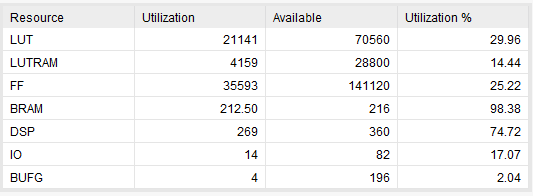
\includegraphics[width=0.9\linewidth]{images/zasoby.png}
    \caption{Zużycie zasobów - zrzut ekranu z programu \emph{Vivado 2019.1}.}
    \label{fig:resources}
\end{figure}
Ostateczne rozwiązanie zostało zaimplementowane ze zrównolegleniem $p = 16$.
Na rysunku \ref{fig:resources} przestawiono zużycie zasobów logiki programowalnej.
Implementacja wykorzystuje niemal wszystkie bloki pamięci \emph{BRAM} oraz znaczą część dostępnych \emph{DSP}.
Uzyskanie ostatecznie lepszych rezultatów jest możliwe, jedynie poprzez bardziej wydajną implementację części programowej.



